%!TEX root=Principal.tex
\chapter{\emph{Proxemcics}}
\label{sec:proxemics}
As pessoas, quando convivem em sociedade, tendem a respeitar o espaço existente entre cada individuo. Esse fenômeno é determinado como espaço social, sendo este medido através da distância social que é um dos princípios fundamentais para uma interação social com qualidade~\cite{Hall:1969, Henkel:2014}. A análise do comportamento das pessoas e a relação da distância social entre os indivíduos foi definido por~\citeonline{Hall:1969} como \emph{Proxemics}. \emph{Proxemics} então pode ser definido com o processo dinâmico de interação entre dois agentes, onde eles fiquem posicionados frente a frente e/ou próximos entre si~\cite{Mead:2011b}.

Durante os estudos de~\citeonline{Hall:1969}, observou-se que a questão da distância social está diretamente ligada a cultura de cada individuo. Isso quer dizer que a percepção dessa distância entre pessoas que viveram em regiões distintas poderá ser diferente. Por exemplo, uma pessoa que vive no Brasil pode não se importar com o indivíduos muito próximos a ele. Em contra partida, a pessoa que vive no Japão talvez tenha preferência por manter uma distância maior entre ele e as demais pessoas durante o processo interação. Além disso, variáveis como gênero e idade também influenciam na relação espacial de interação entre indivíduos.

Apesar da observação sobre as variáveis que podem influenciar na relação da distância social, \citeonline{Hall:1969} não formalizou nenhuma regra sobre a distância social para interações entre indivíduos. Assim, \citeonline{Argyle:1988} definiu quatro zonas de proximidades, formalizando regras para distâncial social nas interações entre indivíduos. São elas: (I) Zona de Proximidade Pública; (II) Zona de Proximidade Social; (III) Zona de Proximidade Pessoal; e (IV) Zona de Proximidade Íntima. A figura~\ref{fig:proximityzones} ilustra a definição de~\citeonline{Argyle:1988} na formalização do espaço social.

\begin{figure}[ht!]
	\centering
	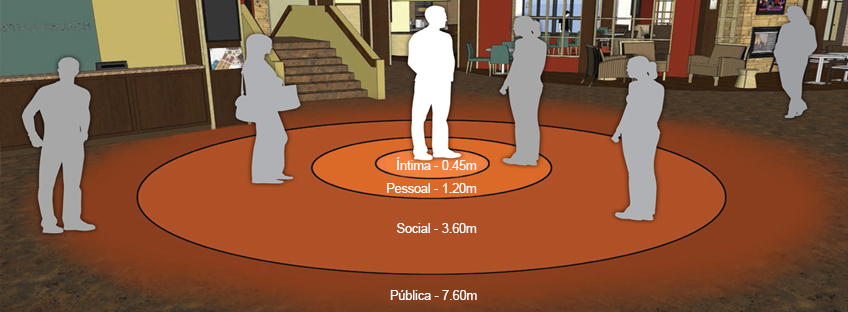
\includegraphics[width=\textwidth]{images/proxemicszones.png}
	\caption{Zonas de Proximidades definido por \citeonline{Argyle:1988}.}
	\label{fig:proximityzones}
\end{figure}

Cada uma das zonas de proximidades apresentadas na figura~\ref{fig:proximityzones} possui características particulares que pode guiar como ocorrerão as interações sociais. Na zona de proximidade social, o individuo pode emitir sons com maior volume do que a zona de proximidade íntima que, por estarem muito próximos os indivíduos acabam se comunicando com sons mais baixos ou até mesmo sussurros. Interações na zona íntima são esperadas normalmente entre amigos muito próximos ou entre casais~\cite{Hall:1969, Argyle:1988}. O comportamento aceitável em zonas de proximidades mais distantes, como a social e a pública, é a comunicação com maior intensidade, movimentos mais amplos e até com uma força física maior que nas regiões mais próximas, onde há a probabilidade maior do indivíduo se assustar com esse tipo de comportamento~\cite{Henkel:2014}.

Além dos comportamentos diferentes em cada zona de proximidade, existe um outro fator que pode atrapalhar a interação exclusiva entre duas pessoas nas regiões mais distantes. A existência de pessoas inseridas nas regiões mais distantes, pode dificultar o estabelecimento uma interação exclusiva devido ao excesso de ruído no cenário. O ruído para esse cenário pode ser considerado através do volume excessivo de pessoas no local, junto com a altura dos sons emitidos e além da quantidade de gestos que cada individuo realiza simultaneamente~\cite{Walters:2009, Henkel:2014}. Isso pode influenciar diretamente no estabelecimento do ponto focal da interação.

Algo que pode ser feito para trabalhar mais próximo do ponto focal da interação é a aproximação entre os agentes, fazendo com que essa interação possua menos ruídos. Para que essa aproximação ocorra com sucesso, alguns fatores são importantes, como velocidade de aproximação, gestos e ruídos emitidos, entre outros fatores. Sendo assim, não é apenas o espaço social que a teoria de \emph{Proxemics} se refere, mas também à análise comportamental. Algumas variáveis que são utilizadas para a leitura corporal também são utilizadas na análise comportamental. \citeonline{Mead:2013} lista algumas variáveis consideradas em seu trabalho, além da distância social, são elas: (I) orientação da postura; (II) orientação do quadril; (III) orientação dos ombros; (IV) posicionamento e orientação da cabeça; e (V) fixação do olhar entre os indivíduos. Todas as variáveis apresentadas por~\citeonline{Mead:2013} auxiliam a determinar a qualidade da interação social entre dois indivíduos, agentes ou entre robôs e humanos.

\emph{Proxemics} tem sido explorado em trabalhos de interação humano-robô~(IHR) desde 1997, somando aproximadamente 25 trabalhos de acordo com~\citeonline{Henkel:2014} e vem crescendo cada vez mais. Contudo, não é apenas em IHR que o tema de \emph{Proxemics} é abordado. Trabalhos relacionados a tecnologia móvel e realidade virtual, também utilizam o tema com o intuito de melhorar a interação dos sistemas de maneira geral. Assim, a próxima seção apresentará os trabalhos relacionados que abordam o tema da \emph{Proxemics} e tecnologias, seguido pela abordagem em IHR, sempre tentando demonstrar o vínculo dos trabalhos apresentados e a tese defendida neste texto.

\section{\emph{Proxemics} e Tecnologia}
\label{sec:proxemicstec}
\citeonline{Hemmert:2013} apresentam um trabalho que tem como objetivo a aplicação de \emph{Proxemics} em aparelhos de telefonia móvel. A ideia principal é fazer com que o telefone reaja de acordo com a aproximação do aparelho pela voz da pessoa. O foco principal dentre as oito variáveis de \emph{Proxemics} é a postura do usuário. Interações de \emph{Proxemics} tem sido um dos modelos gerais em interação humano-computador (IHC). Entretanto, é um tema pouco explorado em telefonia móvel~\cite{Hemmert:2013}.

O projeto utilizado no caso de estudo apresenta uma nova maneira de interagir com dispositivos móveis, em especial telefones, tendo como base variáveis de linguagem corporal e proximidade do indivíduo para com o aparelho. Como trabalho futuro \citeonline{Hemmert:2013} querem apresentar um modelo que faça a leitura de diversas variáveis com o intuito de entender por completo como elas funcionam no comportamento do ser humano.

Um ponto interessante abordado por \citeonline{Hemmert:2013} é quando ele faz refêrencia ao uso de \emph{Proxemics} em IHR. Geralmente os trabalhos de \emph{Proxemics} são voltados ao comportamento de ser humano, e nenhum possui foco na reação do robô, ou seja, como esse robô reagirá caso um ser humano invada o espaço íntimo do robô sem consentimento. Esse é um ponto interessante que deve ser explorado ao longo dessa tese.

No trabalho proposto por \citeonline{Katanis:2012} é apresentado um modelo de aprendizado por reforço aplicado a aproximação de uma pessoa a um avatar em um mundo virtual. O conceito de proximidade é aplicado com o intuito de validar se a tarefa de aproximação foi atingida com sucesso. Apenas 1 participante não alcançou o objetivo de 10, em um dos grupos. Ao todo das 20 pessoas que interagiram com o avatar utilizando aprendizado por reforço, apenas 3 não chegaram a uma posição de zona intima. Não foi avaliado no trabalho de aprendizado por reforço é a melhor técnica para isso, porém o algoritmo Q-Lambda atendeu ao experimento proposto.

\section{\emph{Proxemics} e Interação Humano-Robô}
\label{sec:proxemicsihr}
Nessa seção são apresentados os trabalhos de \emph{Proxemics} aplicados a interação humano-robô~(IHR), como o trabalho de \citeonline{Walters:2009} que propõem um \emph{framework} empírico com o objetivo de auxiliar a detecção da distância real, ou seja, a distância considerando fatores diversos da IHR.

Alguns fatores de impacto na IHR foram apresentados por \citeonline{Walters:2009} na discussão de seu trabalho. Um dos fatores explorados foi o impacto dos sons emitidos pelo robô durante a interação, ou seja, a voz do robô. A voz não causa impacto apenas pelo volume que é emitida, mas também o estilo dela que pode influenciar uma vez que é possível inferir emoções a partir do estilo em que a voz é emitida. Além disso, a voz também pode influenciar no tempo de aproximação entre o robô e o individuo, pois dependendo de como o som é emitido pode gerar insegurança ao individuo que está interagindo com o robô~\cite{Walters:2009}.

Fatores como a aparência do robô e informações demográficas como idade, gênero, grau de instrução, personalidade, carisma, entre outros também podem interferir na IHR. Por exemplo, as pessoas preferem manter uma distância maior dos robôs que possuem uma aparência humanoide, pois ela causa um pouco de preocupação sobre as ações dele, quando comparado a um robô com aparência mais mecânica. Entretanto, a altura do robô não é um fator que apresenta grande relevância para IHR~\cite{Walters:2009}.

Outro trabalho, apresentado por \citeonline{Torta:2011}, tem como objetivo a apresentação de um arquitetura para robótica baseada em comportamento que permite ao robô navegar em segurança por um ambiente doméstico mutável e consiga codificar interações não verbais de maneira embarcada. Dessa maneira, é possível fazer com que o robô possa apresentar o comportamento de aproximação adequado ao seu objetivo, utilizando um novo modelo de espaço pessoal.

Esse novo modelo considera a relação entre a orientação do robô em conjunto com a distância do objetivo e ainda a avaliação do individuo para a orientação de aproximação do robô~\cite{Torta:2011}. Para alcançar esse objetivo \citeonline{Torta:2011} utilizaram um filtro Bayesiano para inferir a localização do objetivo a partir da posição do robô de maneira dinâmica. O filtro Bayesiano é utilizado como guia para o robô em seu algoritmo de navegação.

Nos testes utilizou-se o robô NAO e obteve a validação de que a inclusão do espaço pessoal no algoritmo de navegação trouxe resultados positivos ao modelo implementado. Em estudos futuros, \citeonline{Torta:2011} incluirão outros fatores ao cenário de IHR, como a altura do robô, a aparência e o propósito da interação, e a partir dessas novas variáveis identificar como é possível melhorar a interação de tal forma, que esse modelo obtenha uma qualidade maior em sua aplicação~\cite{Torta:2011}.

A aplicação de \emph{Proxemics} não é exclusiva a robótica social ou doméstica, \citeonline{Srinivasan:2012} aplicam o conceito para o cenário de resgate de vítimas. O trabalho apresentado tem como objetivo avaliar a utilização do olhar social com movimentos de cabeça e funções escalares de \emph{Proxemics} para auxiliar na aproximação e trabalho em regaste de vítimas em centros urbanos.

Nesse cenário o robô deve manter a vítima calma, tranquila, com pensamentos positivos e cuidar dela, na medida do possível, até que o resgate consiga acesso ao local para que o trabalho de extração seja realizado com sucesso~\cite{Srinivasan:2012}. Dois cenários de simulação foram utilizados para validar o método proposto por \citeonline{Srinivasan:2012}. No primeiro cenário observou-se como a vítima correspondia a medida que o robô gesticulava com a cabeça durante a interação comparado ao robô totalmente estático. O movimento da cabeça foi programado para ficar sincronizado com a fala do robô de tal forma, que seu comportamento ficasse próximo a um comportamento natural. Neste primeiro cenário, foi validado a hipótese de que o usuário prefere o robô que tem o movimento social (gesticulação da cabeça) ao invés do robô que permanece totalmente estático durante a interação.

No segundo cenário de simulação, utilizou-se funções escalares para definir a aproximação do robô junto à vítima. Nessa aproximação são consideradas as quatro regiões de proximidades, apresentadas na figura~\ref{fig:proximityzones}, para determinar a interação com a vítima. Foram comparadas três tipos de funções: (I) Logarítmica; (II) Linear; (III) Não escalar. Nos testes os melhores resultados foram obtidos através da função logarítmica, seguida pela função linear e depois a função não escalar~\cite{Srinivasan:2012}. Dessa forma, \citeonline{Srinivasan:2012} esperam melhorar a abordagem com robôs à vítimas de desastres em cenários de centros urbanos.

\citeonline{Okita:2012} realizaram um estudo para identificar quais fatores mais auxiliam na redução da distância física entre o robô e o ser humano. Foram utilizados dois tipos de abordagem para os testes realizados: (I) Robô com a iniciativa de se aproximar do ser humano; e (II) Humano com a iniciativa de se aproximar do robô.

Para o teste de ambos cenários foram utilizados dois tipos de indivíduos, separados em dois grupos diferentes, crianças e adultos. Na execução do teste, \citeonline{Okita:2012} utilizaram o método chamado de \emph{Wizard of Oz} (WOZ) que permite operar o robô através de um controle remoto distante da vista do indivíduo em interação. Dessa forma, é possível passar a impressão de que o robô é autônomo e ao mesmo tempo ter o controle dele para que não ocorra nenhum acidente durante a interação.

O experimento foi executado de duas maneiras diferentes sendo uma o robô aproximar-se sem nenhum tipo de aviso prévio e a outra maneira era exatamente avisar sua aproximação. Observou-se que quando o robô solicitava a permissão para aproximar do individuo o resultado sempre era positivo para a interação, quando comparado à aproximação sem aviso ou com aviso posterior a ação do robô~\cite{Okita:2012}.

Muitos trabalhos apontam maneiras de aplicar o estudo de \emph{Proxemics} em interações sociais. Algumas variáveis que podem afetar a interação são funções interpessoais de relacionamento, fatores fisiológicos moldados pela cultura de origem de um indivíduo, perspectivas etnológicas, além de informações sobre o ambiente de interação, como a luz ambiente, localização e ocupação física do agente, tamanho, entre outros fatores~\cite{Mead:2011b}.

Com a facilidade de compra dos sensores de captura de movimento não invasivo como o Microsoft\textregistered\ Kinect\textregistered ou o PrimeSensor\textregistered, os pesquisadores \citeonline{Mead:2011b} apresentam em seu trabalho um conjunto de métricas que são capazes de auxiliar na automatização do processo de análise do comportamento para distância social. As métricas por eles estabelecidas são: postura, posição do quadril, do ombro, do torso, dos braços, distâncias entre os agentes, gênero, entre outros.

Com base nas métricas definidas foi realizado um estudo conceitual para verificar se o cenário com um Kinect\textregistered\ inserido no ambiente, fosse capaz de capturar todas essas informações para que a partir delas torna-se possível a criação de um mecanismo de análise automática do comportamento de agentes em um ambiente de interação social. Os testes preliminares ocorreram conforme o esperado, possibilitando a validação do cenário apresentado por \citeonline{Mead:2011b}.

Um cenário e ferramenta para coleta de informações sobre indivíduos em interação social são apresentados também por \citeonline{Mead:2011}. O principal objetivo é utilizar as informações coletadas em estudos futuros. Essas informações serviram para a criação de um modelo oculto de Markov (\emph{Hidden Markov Model} (HMM), em inglês) com seis classes para auxiliar na predição das \emph{Proxemics} de interação face a face. Nesse estudo, o HMM demonstrou-se com um desempenho superior para a tarefa de predição, quando comparado com um classificador aleatório ponderado por pesos~\cite{Mead:2011}.

\citeonline{Mead:2012} apresenta uma discussão sobre os tipos de representações para \emph{Proxemics}. Essas representações são: física e psicológica. Além desses dois tipos é proposto uma representação psicofísica que apresenta uma abordagem permitindo unir melhor as qualidades dos outros dois tipos de representação. A representação física tem como objetivo analisar como o espaço social é ocupado por dois indivíduos e é a abordagem mais comum em estudos de \emph{Proxemics}, tanto para interações humano-humano quanto para interações humano-robô. A representação psicológica mantém o foco em fatores de relacionamento interpessoal de alto nível entre dois ou mais indivíduos. Esse fatores estão relacionados a teoria de conflito afiliativo~\cite{Argyle:1965} e também a teoria de adaptação interpessoal~\cite{Burgoon:2007}.

Porém, com as lacunas existentes nesses dois tipos de representação de \emph{Proxemics}, foi proposto o tipo psicofísico. Esse tipo de representação tem como objetivo principal analisar a percepção e a produção de estímulo social entre dois ou mais indivíduos interagindo. A abordagem psicofísica é discutida também por~\citeonline{Hall:1969}. Essa representação está diretamente ligada com a experiência sensorial do estímulo social até os parâmetros espaciais de maneira física. A partir da representação psicofísica é realizado um estudo para capturar informações que servirão de base para treinamento de dois HMM. Cada HMM é responsável por uma exclusiva tarefa, início da interação ou término da interação. Essa representação deve auxiliar nas pesquisas de interação humano-robô, no intuito de que seja possível realizar uma análise para a interação ocorrer com maior qualidade~\cite{Mead:2012}.

Outro trabalho de \citeonline{Mead:2012b} apresenta um mecanismo de análise comportamental através da \emph{Proxemics}. Utiliza-se modelos probabilísticos de tal forma, que seja possível determinar alguns comportamentos dos indivíduos durante uma interação. Como métrica de proximidade utilizou-se a estratégia do mundo de grades para predizer a distância aproximada entre o robô e o individuo. Esse trabalho é implementado através de uma rede Bayesiana dinâmica como uma melhora para o mecanismo~\cite{Mead:2012b}.

Conforme tem sido discutido ao longo dessa seção, para que a interação entre um humano e um robô possa ocorrer de maneira confortável e com qualidade, é necessário que o robô entenda as variáveis de espaço social. Além disso, é necessário também que ele possua o controle sobre essas variáveis de tal forma, que ele consiga tomar decisões sobre as ações que executará~\cite{Mead:2013b}.

\citeonline{Mead:2013b} apresentam um estudo baseado principalmente com variáveis de voz e gestos, utilizando um método de amostragem que tem como entrada a postura do indivíduo ao interagir com o robô. A maior contribuição esperada por \citeonline{Mead:2013b} é a apresentação do entendimento obtido através das interações pré culturais que estão inseridas junto ao estudo de \emph{Proxemics}. O resultado apresentado é apenas uma base de dados para investigar todos os aspectos da interação humano-robô apresentadas no trabalho (voz e gestos).

A partir da base de dados gerada por \citeonline{Mead:2013b}, é apresentado outro trabalho onde \citeonline{Mead:2013} discutem a utilização de um HMM para extração de características comportamentais espaciais do ser humano, em outras palavras, \emph{Proxemics}. Alguns fabricantes de sensores de movimentos, como o Microsoft\textregistered\ Kinect\textregistered\ e o ASUS\textregistered\ Xtion, têm pesquisado técnicas para aprimorar o estudo das distâncias sociais e também seus significados.

Com base nesses estudos, \citeonline{Mead:2013} analisam a possibilidade de automatizar o processo de análise das \emph{Proxemics}. A intenção do trabalho é extrair variáveis para que seja, então, possível determinar o início e o fim de uma interação social através de um HMM. Para realizar os experimentos foram necessários dois indivíduos e um robô aplicados a um cenário de interação, onde os indivíduos se aproximam do robô sendo que os indíviduos estão separados por uma parede. Os resultados são apresentados em relação ao ponto de vista físico e psicológico. Na detecção das variáveis que representam as \emph{Proxemics} de maneira dinâmica, \citeonline{Mead:2013} consideram os resultados satisfatórios e como sequência do trabalho é mantido o foco em interações com fatores psicológicos complexos, para aprimorar a precisão do \emph{framework} criado.

\citeonline{Mead:2014} direcionam o foco de seu trabalho para a análise de conversa social e gestos, tanto na questão de produção das conversas e gestos de maneira automática quanto para o reconhecimento, aplicados em interações humano-humano e humano-robô. Todo o trabalho realizado está relacionado com o estudo de \emph{Proxemics} na interações sociais, uma vez que essas tem o objetivo de não só identificar as variáveis, mas também de interpretar, manipular e compreender a dinâmica do comportamento espacial dentro do cenário das interações sociais.

Os estudos e experimentos sociais realizados por \citeonline{Mead:2014} auxiliaram na coleta de informações sobre o volume da fala de acordo com a distância, além dos gestos que necessitam de espaços maiores para execução sem prejudicar a interação. Os resultados apresentados apontam que a distância de interações entre humanos é menor que a distância da interação entre um humano e um robô. Além disso, os resultados obtidos não são aplicados à múltiplas culturas (nesse caso origem dos indivíduos), e isso deve ser realizado em outros trabalhos segundo \citeonline{Mead:2014}. Um mecanismo para personalizar o tratamento que o robô terá com o indivíduo durante a interação também é algo de deve ser construído ao longo dos trabalhos futuros.

Analisando a diferença de cultura para variáveis de \emph{Proxemics}, \citeonline{Eresha:2013} apresentam como objetivo do trabalho a avaliação do comportamento de indivíduos ao se encontrarem com dois robôs interagindo entre si e caminhando em direção ao individuo de tal forma que este possa também interagir ou não com os robôs conforme se aproximam. Além de avaliar o comportamento dos indivíduos durante a interação com os robôs, \citeonline{Eresha:2013} adicionaram a variável de cultura ao estudo. O objetivo é identificar como é a diferença de comportamento entre culturas diferentes. Foram escolhidos participantes de origem árabe e alemã para o estudo.

Nos experimentos, \citeonline{Eresha:2013} utilizaram dois robôs NAO que se posicionavam a 40 cm de distância entre eles e caminhavam até ficarem a uma distância diagonal de 85 cm do indivíduo. Para o experimento houve a participação de 24 indivíduos, 12 árabes e 12 alemães, sendo metade do gênero feminino e a outra metade do gênero masculino. Os testes apresentaram resultados interessantes, pois alguns indivíduos não reagiram como o esperado para pessoas de sua origem e muitas vezes o comportamento social na interação era idêntico entre alemães e árabes. Outro ponto apresentado por \citeonline{Eresha:2013} é que durante os testes dois alemães apresentaram o sentimento de medo de serem atacados fisicamente pelos robôs.

O trabalho de \citeonline{Eresha:2013} apresenta indícios de que as variáveis de \emph{Proxemics} não estão ligadas a cultura do indivíduo, como origem, mas sim na experiência cultural que este teve ao longo de sua vida. Dessa maneira, pode-se dizer que \emph{Proxemics} são variáveis extraculturais, porém é necessário realizar um tratamento para esse tipo de condição de tal forma, que o robô possa interagir com mais qualidade com pessoas que possuem diferentes experiências culturais.

\citeonline{Henkel:2012} investigam características entre diversas plataformas de teste para interação humano-robô, e com base no resultado deste estudo é realizado a proposta de uma nova plataforma de testes. A nova plataforma foi desenvolvida, pois \citeonline{Henkel:2012} alegam que não existe nenhuma plataforma de teste capaz de atender aos seis atributos de dependência das \emph{Proxemics}. Os atributos são: (I) movimento afetivo; (II) leitura das \emph{Proxemics}; (III) interação de voz; (IV) manipulação do estilo de áudio; (V) controle do olhar; e (VI) apresentação de conteúdo através de mídia, por exemplo, monitor ou leds.

A plataforma é constituída por uma cabeça feita com um monitor de 7'', junto com um encaixe construído para ser acoplado em qualquer base de robôs já existentes no mercado. Alguns testes que foram realizados no cenário de resgate à vítimas demonstram que as pessoas que tinham a zona de espaço social íntimo invadida por qualquer parte do robô sem uma interação prévia ficavam em situação de \emph{stress} elevado. Essa reação foi totalmente oposta quando o robô iniciava com qualquer tipo de interação antes de realizar a aproximação do indivíduo~\cite{Henkel:2012}. O primeiro contato antes da aproximação para uma interação maior é importante, pois esse comportamento pode definir o quão confortável a interação entre os agentes será e esse comportamento deve ser explorado durante a execução dessa tese.

Em outro trabalho, \citeonline{Henkel:2014} apresentam duas funções escalares para avaliar os valores de proximidade entre humanos e robôs. As funções escalares são comparadas com outras funções não-escalares e também entre si de tal forma, que seja possível uma tomada de decisão em tempo de execução da ação/interação. As duas funções escalares apresentadas são: (I) logarítmica; e (II) linear.

Os testes foram executados no cenário de regaste à vitimas. Quando a função logarítmica foi aplicada, os resultados apresentados foram melhores do que os obtidos com as demais funções. Como o principal objetivo de \citeonline{Henkel:2014} é generalizar o método para outros cenários, eles pretendem realizar testes do modelo em outras situações e também utilizando outros tipos de robôs para sustentar melhor a hipótese. Os estudos prévios realizados demonstram que a generalização do modelo é possível.

A integração social do robô com os ambientes que envolvem cenários de cuidados médicos, construção, educação, serviço públicos, entre outros pode ser a chave de sua aceitação por parte dos seres humanos. Um dos caminhos para conseguir esse objetivo é fazer com que o robô saiba ter um comportamento adequado de interação em cada um desses cenários, assim como o que já é demonstrado em filmes de ficção científica. Dessa maneira, é possível fazer com que os seres humanos utilizem o próprio senso social para identificar essas habilidades no robô, quebrando um pouco o medo de interagir com ele~\cite{Heenan:2014}.

Como primeiro passo para que a interação ocorra naturalmente entre o ser humano e o robô, \citeonline{Heenan:2014} acreditam que deve haver sempre uma saudação entre ambas partes logo ao primeiro contato. Esse tipo de comportamento pode ser fundamental para que haja uma aceitação social do robô entre as pessoas. Durante uma saudação existem diversos fatores que são analisados implicitamente pelo ser humano, como nuanças de comunicação não verbal, vocalização das palavras e a distância inter pessoal. Esses fatores devem ser considerados ao projetar uma saudação por parte do robô, fazendo com que seja possível o robô iniciar a interação.

Fazer com que um robô realize uma saudação natural não é uma tarefa muito fácil. Deve ser considerado que um robô não tem a mesma capacidade de identificar as nuanças sociais com a mesma velocidade de um ser humano. Outro ponto negativo é que o robô possui o lado mecânico limitado, quando comparado a musculatura do ser humano. Assim, o primeiro objetivo do trabalho de \citeonline{Heenan:2014} é definir um subconjunto exato de elementos de uma saudação social que possa ser articulado pelo robô durante a tarefa e ainda como implementar as sutilezas do comportamento da interação de saudação social.

Os testes executados demonstram que a saudação é um ponto importante para o resultado com sucesso da interação com o ser humano. O robô NAO utilizado nos testes foi capaz de implementar ações de comportamento como o contato visual, linguagem corporal e distância social para comunicação efetiva. Apesar de algumas restrições do modelo de saudação ocorrerem devido a limitação do NAO, é possível realizar a generalização do mesmo para outros robôs~\cite{Heenan:2014}.

Percebeu-se que o contato visual se apresentou como um elemento de interação social bem natural, contudo deve-se tomar cuidado para que o robô não fique encarando a pessoa constantemente, pois é gerado um desconforto para a pessoa durante o contato. \citeonline{Heenan:2014} dizem que é possível afirmar que utilizar a saudação é importante no primeiro contato de dois agentes, além de aumentar a capacidade da interação social entre o robô e o ser humano.

\citeonline{Vazquez:2014} apresentam um robô móvel no formato de mobília, chamado Chester, construído para realizar interações com crianças. Como o Chester é muito grande optou-se por usar um segundo robô não móvel, ao qual \citeonline{Vazquez:2014} denominam \emph{sidekick}. O \emph{sidekick} é como um parceiro ou personagem secundário que auxilia as pessoas em volta a prestarem atenção no personagem principal, como por exemplo o burro da animação Shrek. O \emph{sidekick} criado é um abajur chamado Blink. Ele fica acoplado em cima do Chester. A figura~\ref{fig:vazquez} apresenta a combinação dos robôs Chester e Blink.

\begin{figure}[ht!]
	\centering
	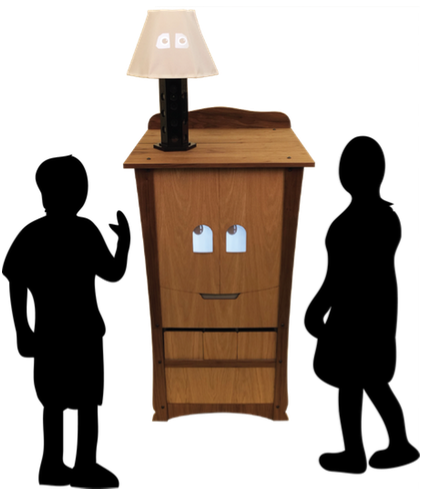
\includegraphics[width=0.4\textwidth]{images/vazquez2014.png}
	\caption{Chester e Blink os robôs apresentados por \citeonline{Vazquez:2014}.}
	\label{fig:vazquez}
\end{figure}

Blink tem uma linguagem própria e apenas o Chester é capaz de entender. É como o R2D2 em Star Wars que apenas alguns personagens são capazes de compreende-lo e falar com ele diretamente. Os resultados obtidos mostram que a inserção de um \emph{sidekick} não altera a questão de proximidade das crianças em relação ao robô, mas melhora a atenção com os elementos falantes do cenário~\cite{Vazquez:2014}.

Foi possível caracterizar alguns comportamentos das crianças ao interagir com os robôs. É afirmado por \citeonline{Vazquez:2014} que o formato de mobília para robôs é plausível para utilizar em robôs que interagem com crianças, pois elas se sentem mais empáticas aos robôs. Contudo, é questionável essa afirmação. Será que o que realmente influenciou esse resultado foi o formato do robô ou foi seu comportamento durante o contato com as crianças? Provavelmente, esse é um resultado que pode ser obtido com a mistura desses dois fatores, aparência e comportamento.

Por questões de segurança os testes foram executados utilizando o método \emph{Wizard of Oz} (WoZ), onde existe um especialista controlando o robô através de um controle de videogame, por exemplo. Foram conduzidos duas variantes do teste, são elas: (I) com o \emph{sidekick} ativo; e (II) com o \emph{sidekick} inativo. O especialista que controla o robô encontrava-se na mesma sala de teste, mas algumas precauções foram consideradas para que não houvesse ruído nos resultados do teste. Uma dessas precauções foi inseri-lo na sala do teste antes do mesmo iniciar para que aparenta-se que ele estava apenas trabalhando normalmente. Além disso, o controle do robô foi posicionado embaixo da mesa para facilitar a oclusão do objeto e ainda fez com que nenhuma criança notasse que o robô era teleoperado por um especialista~\cite{Vazquez:2014}.

Para capturar as informações de distância foi acoplado ao teto um sensor Microsoft Kinect. Ele é responsável por capturar as informações de distância entre o robô e a criança interagindo com ele. Notou-se que na maioria das vezes a criança ficava sempre de frente a face do robô e não ao seu lado ou atrás dele. Variáveis como o tempo de resposta para se afastar enquanto o robô dizia ``recue'' também foi considerado para identificar os resultados~\cite{Vazquez:2014}.

Nos resultados finais, \citeonline{Vazquez:2014} encontraram algumas limitações do robô e também do experimento, como por exemplo, o pouco conteúdo de linguagem que o robô possui implementado para dar respostas aos participantes do teste. Outro problema encontrado foi no início e no final de interação onde outros pontos do cenário e tarefa atrapalharam a coleta de informações ou melhor o foco do caso de estudo. Devido a esse problema, a utilização de um \emph{sidekick} deverá ser estuda com mais detalhes e realizar os testes novamente para que possa ser comprovado o real benefício dele nos resultados da interação. Resultados preliminares confirmam que o \emph{sidekick} não atrapalha na interação entre o robô principal e as pessoas e ainda auxilia a aumentar a atenção das pessoas o que auxilia em um melhor comportamento reativo dos participantes~\cite{Vazquez:2014}.

Alguns estudos utilizando robôs para interagir com crianças com autismo apontam que pode apresentar reações positivas e negativas para o âmbito social. Especialistas são capazes de identificar esse tipo de avaliação através da análise dos vídeos gravados entre sessões. O objetivo do trabalho de \citeonline{Feil-Seifer:2010} é automatizar esse processo de análise através do uso de robôs. Para isso foi desenvolvido um classificador heurístico para discretizar as crianças que conseguem interagir com o robô daquelas que não conseguem.

O cenário de teste é composto de uma sala, um robô totalmente autônomo com o objetivo de incentivar a interação, uma criança diagnosticada com autismo e um familiar mais próximo. Para incentivar a interação o robô deve se aproximar apresentando vocalizações de sons felizes e também esboçar um sorriso para a criança, por exemplo. Caso alguma criança se afaste do robô, ele deve esboçar uma face triste e emitir sons que demonstre a sua não felicidade~\cite{Feil-Seifer:2010}.

Durante os testes foram gravados vídeos e algumas marcações foram realizadas no robô, e nos pais, com o intuito de auxiliar na medida das distâncias entre a criança e o robô ou seus pais. Para realizar uma avaliação sobre esse cenário foi utilizada a seguinte heurística: Para cada trecho de tempo se a criança encontrar-se a 0,85 m dos pais ela é considerada próxima à eles. Caso ela encontra-se a 0,5 m de uma parede ela é considerada próxima a parede. Para ser considerada atrás do robô ela deveria estar a qualquer distância, mas entre uma angulação maior que 135º e menor que -135º~\cite{Feil-Seifer:2010}.

A partir das informações capturadas é possível gerar o classificador onde ele análise se pelo menos 50\% do tempo gasto é com as informações de comportamento negativo (mapeado pelas heurísticas), então é considerado que a criança não deseja interagir com o robô. Caso contrário, menos de 50\% do tempo gasto, a criança deseja interagir com o robô. Apesar dos resultados positivos, esse classificador não deve ser considerado como regra para que haja uma maior escalabilidade do projeto e sua aplicação~\cite{Feil-Seifer:2010}. Esses tipos de parâmetros podem auxiliar na determinação de interação ou não interação. Dessa forma, pode-se fazer com que o robô recue ou tente uma nova abordagem, para quando a reação do indivíduo for negativa.

Outros estudos confirmam a existência de uma relação de distância social entre o robô e o ser humano, entretanto nenhum método foi proposto computacionalmente para que haja uma geração do comportamento em relação a essa distância~\cite{Henkel:2012b}. Assim, é apresentado um método escalar do comportamento do robô de tal forma, que esse comportamento baseado na distância social tenha como suporte uma lei física e duas psicológicas: \emph{inverse-square law}, \emph{Weber-Fechner law} e \emph{Steven's Power law}~\cite{Henkel:2012b}.

O cenário de teste é um ambiente de desastre no qual o robô deve localizar a vítima. A interação ocorre por meio de voz sintetizada, caminhos pre definidos e controle segundo o módulo de teste WoZ. Como meio de avaliação questionários pré e pós interação são aplicados aos usuários que participam do teste~\cite{Henkel:2012b}.

Atributos primários foram determinados para que possam ser identificados alguns níveis de consistências sociais: conforto, movimentos naturais, consideração do espaço pessoal, segurança e controle próprio. Atributos secundários também foram considerados nos estudos de \citeonline{Henkel:2012b}, são eles: atenciosidade, empatia, felicidade, similaridade, inteligência, sensibilidade, submissão e confiança. Os resultados demonstram que todos atributos primários e apenas três secundários provaram que apresentam melhor significância para o processo. O sistema de percepção escalar provou ser melhor do que o não escalar. O modelo escalar linear apresentou o mesmo resultado que o não escalar~\cite{Henkel:2012b}.

Um dos pontos chave dos trabalhos apresentados ao longo dessa seção é que sempre utilizam sensores no ambiente para medir as variáveis de \emph{Proxemics} entre a pessoa e o robô. Contudo, acredita-se que esse tipo de abordagem não é natural ao robô móvel, pois os seres humanos não tem o auxílio sendo assim o robô também não deve utilizar desses recursos. Contudo, as variáveis de \emph{Proxemics} se mostram essenciais para determinar o sucesso de uma interação ou não, e devem ser consideradas ao longo da proposta desta tese de doutorado.

Dessa forma, todas as variáveis apresentadas nos trabalhos dessa seção são importantes para avaliar o comportamneto de um indivíduo durante uma interação com robôs e até outros dispositivos tecnológicos. Na seção~\ref{sec:extracaocaracteristicas} são apresentados as variáveis consideradas para o desenvolvimento desse trabalho. Além das variáveis, também são avaliados os meios de captura das informações visando a aplicação do trabalho desenvolvido na tese inserido em um ambiente inteligente.
